\section{The work and its place in the institute: description and analysis}
\label{sec:work}

\subsection{Role, contribution and working environment}
\label{sec:setup}

In the team's workflow I acted as an investigator inside an existing code base.
SMILify supplied the parametric representation and a baseline
optimisation-based fitting pipeline; I added the diagnostic and validation
machinery around it and the extensions evaluated with it
(Table~\ref{tab:contrib}). Every extension was judged against a criterion
registered before the experiment, so that a favourable-looking result could
not be reinterpreted afterwards. The stack is Python, PyTorch, PyTorch3D~\cite{pytorch3d},
Trimesh, Blender and a CGAL-based Alpha Wrap, with YAML-configured experiments
under Git, run as batch jobs with recorded seeds and preserved checkpoints on
JURECA and on an RWTH GPU allocation.

\begin{table}[!htb]
\centering
\caption{Components of the repository I implemented or extended.}
\label{tab:contrib}
\begin{tabular}{@{}L{0.36\linewidth}L{0.56\linewidth}@{}}
\toprule
\textbf{Component} & \textbf{Contribution}\\
\midrule
Preprocessing & Implemented and extended (Alpha Wrap, ManifoldPlus, cleanup,
 quadric-error reduction)\\
Joint limits & Integrated into the 3D registration path\\
Synthetic correspondence benchmark & Implemented\\
Learned pose initialisation & Integrated and evaluated\\
SDF analysis, learned descriptors & Implemented and evaluated\\
Evaluation harness, Joint Alignment Benchmark & Designed and implemented\\
HPC pipeline & Configured on two systems\\
Morphometric analysis & Implemented\\
\bottomrule
\end{tabular}
\end{table}

\subsection{The model and what the objective observes}
\label{sec:framework}

The model has a fixed-topology template of $10{,}235$ vertices, a kinematic
tree of $55$ joints, per-vertex skinning weights, a $25$-dimensional shape
basis, a bilateral symmetry map and authored joint rotation limits. Fixed
topology is what makes correspondence meaningful: vertex $i$ denotes the same
anatomical locus in every fit, so a registered corpus lives in one coordinate
system. A shaped vertex $\bar{\mathbf v}_i(\bm\beta)=\mathbf v^{0}_i+\sum_k\beta_k\mathbf s_{ik}$
is posed by linear blend skinning,
\begin{equation}
\mathbf v_i(\bm\beta,\bm\theta)=\sum_{j=1}^{55} w_{ij}\,G_j(\bm\theta)\,\bar{\mathbf v}_i(\bm\beta),
\qquad G_j(\bm\theta)=\prod_{k\in\mathrm{anc}(j)}\big[R(\theta_k)\,|\,\mathbf t_k\big].
\label{eq:lbs}
\end{equation}
Two consequences drive later results. A rotation error at a proximal joint
changes $G_j$ for every descendant and so displaces everything distal to it.
And the surface depends on joint \emph{positions} only through $G_j$, so a
surface can look right while the skeleton inside it is wrong.

The pipeline (Figure~\ref{fig:pipeline}) has four stages: preprocessing,
initialisation, registration and, new in this work, a correspondence-audit
stage that reports how far each vertex's identity can be trusted rather than
only how close the surfaces are.

\begin{figure}[!htb]
\centering
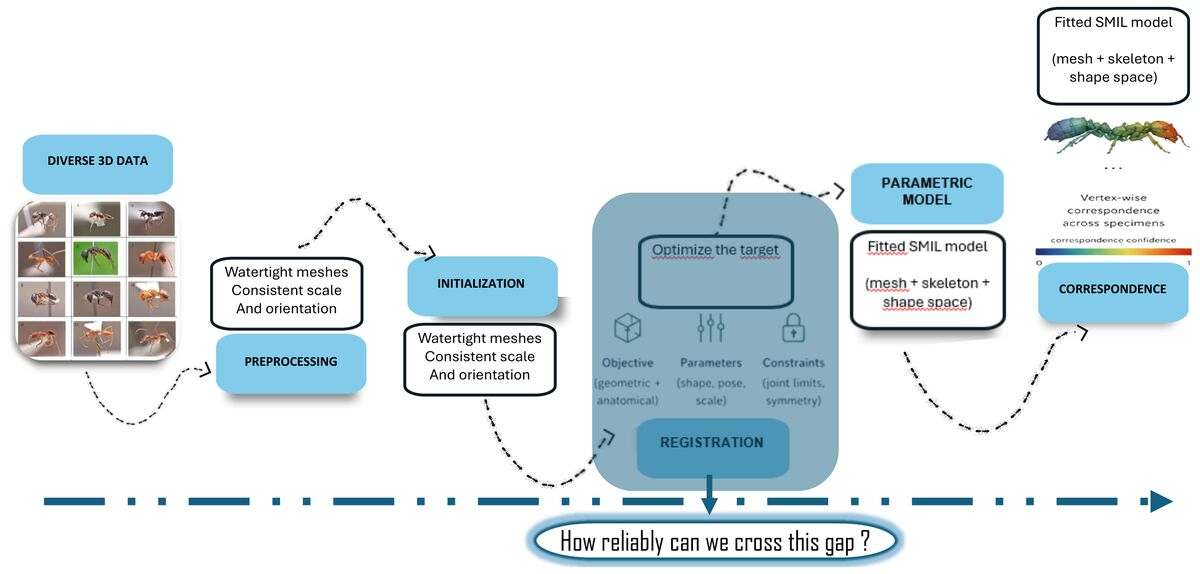
\includegraphics[width=0.8\linewidth]{figures/fig_pipeline_full.jpg}
\caption[The registration pipeline]{The registration pipeline, from diverse
raw scans to a fitted parametric model with vertex-wise correspondence. The
correspondence stage did not exist before this work.}
\label{fig:pipeline}
\end{figure}

\paragraph{The objective.} Let $X$ and $Y$ be area-weighted point samples
($N=6000$ each) of the model surface $V=S(\bm\beta,\bm\theta,s)+\mathbf d$ and of
the scan $T$, where $S$ is the skinned shape of Equation~\eqref{eq:lbs} and
$\mathbf d$ the free per-vertex deformation. The registration objective is
\begin{equation}
\mathcal L=\underbrace{w_{\mathrm{ch}}\mathcal L_{\mathrm{ch}}+w_{\mathrm n}\mathcal L_{\mathrm n}}_{\text{observe the target}}
+\underbrace{w_{\mathrm e}\mathcal L_{\mathrm e}+w_{\Delta}\mathcal L_{\Delta}+w_{\mathrm o}\mathcal L_{\mathrm o}}_{\text{regularise the mesh}}
+\underbrace{w_{\mathrm m}\mathcal L_{\mathrm m}+w_{\mathrm{sym}}\mathcal L_{\mathrm{sym}}+w_{\ell}\mathcal L_{\ell}+w_{\sigma}\mathcal L_{\sigma}}_{\text{priors on the model}},
\label{eq:objective}
\end{equation}
with the symmetric Chamfer term
$\mathcal L_{\mathrm{ch}}=\frac1N\sum_{x\in X}\min_{y\in Y}\|x-y\|^2+\frac1N\sum_{y\in Y}\min_{x\in X}\|x-y\|^2$,
the mean squared edge length $\mathcal L_{\mathrm e}$ (a shrinkage regulariser),
the uniform Laplacian $\mathcal L_{\Delta}$, and the deformation penalty
$\mathcal L_{\mathrm o}=\frac1{|V|}\sum_v\|\mathbf d_v\|^2$. The model priors keep
the midsagittal vertex set on the symmetry plane ($\mathcal L_{\mathrm m}$), tie
left to right ($\mathcal L_{\mathrm{sym}}$), penalise joint rotations outside the
authored box with a hinge that is flat inside and linear outside
($\mathcal L_{\ell}$), and bound per-joint scale beyond a free band of a factor
two with $\mathcal L_{\sigma}=\operatorname{mean}\,(|\ln s_{jk}|-\ln 2)_+^2$. This
last term, the scale barrier, is a soft penalty by design: a hard clamp would
put a gradient discontinuity exactly where difficult specimens live.
Table~\ref{tab:objective} states what each term \emph{observes}, which is the
information the optimiser actually has.

\begin{table}[!htb]
\centering
\caption{Terms of the registration objective and what each one observes.}
\label{tab:objective}
\begin{tabular}{@{}L{0.26\linewidth}L{0.66\linewidth}@{}}
\toprule
\textbf{Term} & \textbf{What it observes}\\
\midrule
$\mathcal L_{\mathrm{ch}}$, $\mathcal L_{\mathrm n}$ & The scan as a point set with normals; a function of two surfaces,
 blind to which vertex is which\\
$\mathcal L_{\mathrm e}$, $\mathcal L_{\Delta}$, $\mathcal L_{\mathrm o}$ & Mesh regularity and the size of the
 residual deformation (ARAP-style~\cite{arap}); independent of the target\\
$\mathcal L_{\mathrm m}$, $\mathcal L_{\mathrm{sym}}$ & Bilateral consistency of the model\\
$\mathcal L_{\ell}$, $\mathcal L_{\sigma}$ & Joint \emph{angles} and per-joint scales against authored ranges\\
\bottomrule
\end{tabular}
\end{table}

No term takes a joint location or a vertex identity as an observation. The
next subsection turns this observation into a precise statement about what can
and cannot be recovered.

\subsection{What the objective can and cannot identify}
\label{sec:formal}

Two elementary properties of Equation~\eqref{eq:objective} organise every
experiment that follows.

\textbf{Label invariance of the data terms.} The target-dependent terms
$\mathcal L_{\mathrm{ch}}$ and $\mathcal L_{\mathrm n}$ depend on $V$ only through
the point set and its normals. For any permutation $P$ of the vertex index,
$\mathcal L_{\mathrm{ch}}(PV,T)=\mathcal L_{\mathrm{ch}}(V,T)$: the data cannot
distinguish a solution from one that assigns the same surface to different
anatomical labels. Identity can therefore enter only through the structure of
the model's image (fixed topology, skinning, symmetry, limits), so
identifiability is a property of the \emph{model and its priors}, not of the
data term. This is why a lower Chamfer distance carries no information about
vertex identity.

\textbf{Pose--deformation equivalence.} Because the deformation is added after
skinning, $V=S(\bm\beta,\bm\theta,s)+\mathbf d$, any alternative pose
$\bm\theta'$ reproduces exactly the same surface with
$\mathbf d'=\mathbf d+S(\bm\beta,\bm\theta,s)-S(\bm\beta,\bm\theta',s)$. The
data terms, and the edge and Laplacian terms, which also depend only on $V$,
are constant along this family. Among the pose-dependent terms only three
distinguish its members: the deformation penalty $\mathcal L_{\mathrm o}$, the
joint-limit hinge $\mathcal L_{\ell}$ and the symmetry priors. The pose
estimate is therefore
\begin{equation}
\hat{\bm\theta}=\arg\min_{\bm\theta'}\;w_{\mathrm o}\,\frac1{|V|}\big\|S(\bm\beta,\bm\theta,s)-S(\bm\beta,\bm\theta',s)+\mathbf d\big\|^2+w_{\ell}\mathcal L_{\ell}(\bm\theta')+\cdots,
\label{eq:gauge}
\end{equation}
that is, \emph{the pose that needs the least deformation}. This is a prior,
not an observation, and it recovers the true pose exactly when the unmodelled
part of the scan is small relative to the displacement a pose error induces
(true for model-generated targets, where $\mathbf d^\ast=0$; not guaranteed for
real specimens). Figure~\ref{fig:gauge} shows the consequence: as
$w_{\mathrm o}$ decreases the loss along the family flattens, the pose becomes
underdetermined, and small contributions from the other terms decide where
the optimiser stops. The two predictions are exactly what the experiments find:
lowering the deformation penalty buys surface fit at the cost of the skeleton
(Section~\ref{sec:geometric-agreement}), and pose error that the objective
cannot see persists at joints where attachment is set jointly by pose, scale and
shape (Section~\ref{sec:articulation}).

\begin{figure}[!htb]
\centering
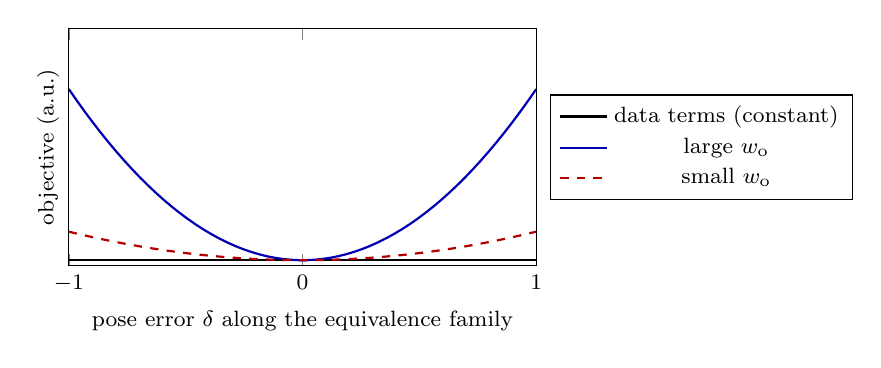
\begin{tikzpicture}
\begin{axis}[width=0.62\linewidth,height=4.6cm,xlabel={pose error $\delta$ along the equivalence family},
 ylabel={objective (a.u.)},xlabel style={font=\footnotesize},ylabel style={font=\footnotesize},
 tick label style={font=\footnotesize},legend style={font=\footnotesize,at={(1.03,0.5)},anchor=west},
 domain=-1:1,samples=60,ymin=0,ymax=1.25,xmin=-1,xmax=1,xtick={-1,0,1},ytick=\empty]
\addplot[thick,black] {0.03};
\addplot[thick,blue!70!black] {0.9*x^2+0.03};
\addplot[thick,red!70!black,dashed] {0.15*x^2+0.03};
\legend{data terms (constant), large $w_{\mathrm o}$, small $w_{\mathrm o}$}
\end{axis}
\end{tikzpicture}
\caption[Pose--deformation equivalence]{Schematic of Equation~\eqref{eq:gauge}.
Along the family of poses that reproduce the same surface, the data terms are
constant and only the deformation penalty (and the limits) vary. A large
penalty gives a well-conditioned minimum at the true pose ($\delta=0$); a small
one leaves a nearly flat valley in which the pose is set by whatever else
differs between candidates.}
\label{fig:gauge}
\end{figure}

\textbf{From retrieval to assignment.} The same logic separates two tasks that
are easily conflated. A descriptor $f$ supports \emph{retrieval},
$\pi(j)=\arg\min_i\|f(t_j)-f(v_i)\|$, which is a relation: nothing forces $\pi$ to
cover the template or to be consistent across points. A dense correspondence
needs an \emph{assignment}, a coupling $P$ between template and target with
controlled marginals, as in optimal transport,
$\min_{P\in\Pi(\mu,\nu)}\langle P,C\rangle-\varepsilon H(P)$~\cite{ot}, whose
marginal constraints are exactly what enforces coverage and whose unbalanced
variants accommodate incomplete scans. The measured coverage of a retrieval
field (Section~\ref{sec:learned-correspondence}) is therefore not an
implementation detail but the quantity that separates the two tasks.

\subsection{The shipped algorithm: hierarchical placement and surface refinement}
\label{sec:algorithm}

The shipped recipe is organised to supply, step by step, the information the
objective lacks, without adding an observation of identity
(Table~\ref{tab:stages}). Six identical legs make a global Chamfer term
multimodal: any leg can be matched by any leg's surface. The body, by contrast,
is three blobs on an axis and is essentially unimodal. The recipe exploits this
asymmetry. A body-only stage places the body and, with it, the six coxae; the
target is then partitioned by anatomical territory and each leg chain is fitted
against only its own assigned points; all joints are then released with the
partition kept; and only then do the surface stages free pose, shape, scales
and deformation together under the regularisers of
Equation~\eqref{eq:objective}, with the deformation penalty deliberately
expensive so that deformation absorbs genuine species detail and not pose error.
The partition supplies \emph{regional} identity (which leg), never
within-region location, which is why it resolves the multimodality yet leaves
the problem measured in Section~\ref{sec:oracle}.

\begin{table}[!htb]
\centering
\caption{Stages of the shipped registration recipe.}
\label{tab:stages}
\begin{tabular}{@{}L{0.14\linewidth}L{0.25\linewidth}L{0.27\linewidth}L{0.25\linewidth}@{}}
\toprule
\textbf{Stage} & \textbf{Moves} & \textbf{Observes} & \textbf{Purpose}\\
\midrule
H0 body & Body chain; legs frozen & Global Chamfer & Place body and coxae\\
H1 legs & Leg chains; body frozen & Own-territory points per leg &
 Remove six-leg multimodality\\
H2 joints & All joints; partition kept & Partitioned Chamfer & Refine without
 cross-leg matching\\
Surface, coarse & Pose, shape, scales, $\mathbf d$ (1000 it., $w_{\mathrm o}=5$) &
 Symmetric Chamfer, 6000 samples & Fit surface; deformation expensive\\
Surface, fine & Same, smaller steps (1000 it., $w_{\mathrm o}=2$) & Chamfer weight
 halved, regularisers relaxed & Absorb residual detail\\
\bottomrule
\end{tabular}
\end{table}

The difficulties met here are recognised in the registration literature.
Deep Closest Point~\cite{dcp} learns point embeddings for closest-point
matching, PREDATOR~\cite{predator} predicts the overlap of low-overlap pairs,
and GeoTransformer~\cite{geotransformer} combines geometric attention with
coarse-to-fine matching; functional maps~\cite{fmaps} and optimal
transport~\cite{ot} offer globally consistent correspondence formulations. This
work studies a harder, model-based variant: registration constrained to the
image of an articulated parametric model, where nearest-surface matching is the
local mechanism and the open question is what information it lacks.

\subsection{Experimental design: how a latent explanation can be checked}
\label{sec:method}

Because the quantity of interest is never observed, every claim rests on one of
two kinds of ground truth, and the design is organised around knowing which.

\textbf{Synthetic ground truth.} The model can generate its own targets: sample
$(\bm\beta,\bm\theta)$, pose the template, export an anonymous mesh
(optionally degraded), refit it with the production fitter, and compare fitted
vertex $i$ with true vertex $i$. This gives exact correspondence error at no
annotation cost and allows one factor at a time to be changed. Its scope is exact
identity: because the target comes from the model, it isolates the inverse
problem from data quality and gives a lower bound for real scans, while
correctness on real specimens is established by the expert benchmark.

\textbf{Expert ground truth.} For real specimens an expert placed 3D joints
manually, and a Joint Alignment Benchmark (JAB) was built on them: 11
specimens, 12 strategies, 3 optimiser seeds, 396 fits, pre-registered and
frozen with a SHA-256 hash before any strategy was run, with error reported as
a percentage of Weber's length (WL, a posture-independent body-size unit).
Auditing this ground truth was itself a finding (\F{F7}). Earlier joint errors
had been measured in a reference frame fitted \emph{to the production
skeleton}, an error of the fiducial-registration type that is known to be
uncorrelated with the error at the points that matter~\cite{fitzpatrick};
re-registering the annotations through each scan mesh moved the apparent
production error from $42.7\%$ to $25.1\%$ of WL without touching the fitter.
Four annotation scenes were mirror images and were corrected; one specimen
had been annotated on another specimen's mesh and was excluded; and
surface-landmark coordinates stored in Blender's frame needed the axis map
$(x,y,z)\mapsto(x,z,-y)$, so earlier surface-landmark analyses were discarded.
The lesson is a general one: ground truth is part of the measurement system, and
a mis-specified reference frame produces confidently wrong numbers.

\textbf{Evaluation protocol.} A metric that a targeted attack can improve by
damaging the mesh cannot be the sole judge of a fit: snapping distal vertices
onto the nearest target surface improves a per-part distance by $53\%$ while
edge-length distortion rises $7.5$-fold. The protocol therefore combines three
levels (Table~\ref{tab:levels}), and an intervention is adopted only if it does
not degrade levels 1--2 and is checked at level 3 wherever ground truth exists.
Because the benchmark is small, inference is made at the specimen level with
Hodges--Lehmann shifts, Holm correction and Friedman ranking~\cite{demsar},
and a strategy is called \emph{equivalent} only if its confidence interval lies
inside the measured annotation repeatability ($\pm2.5\%$ WL), following the
logic of equivalence testing~\cite{lakens}. At $n=11$ the pre-registered
specimen-level test resolves effects that are consistent across about ten of
eleven specimens; smaller or less consistent effects are reported with their
intervals and with a joint-level mixed model, which has the power to resolve
them.

\begin{table}[!htb]
\centering
\caption{The three evidence levels of the evaluation protocol, always used
together.}
\label{tab:levels}
\begin{tabular}{@{}L{0.22\linewidth}L{0.40\linewidth}L{0.30\linewidth}@{}}
\toprule
\textbf{Level} & \textbf{Metrics} & \textbf{Question answered}\\
\midrule
1. Surface proximity & Chamfer, F-score, per-part variants & Does the mesh
 cover the target?\\
2. Integrity & Edge-length distortion, Laplacian and ARAP deviation, normal
 consistency & Was coverage bought by damaging the mesh?\\
3. Anatomical truth & Synthetic vertex-identity error; expert joint error &
 Is vertex $i$ on the locus it represents?\\
\bottomrule
\end{tabular}
\end{table}

\textbf{Metrics.} On synthetic data the correspondence accuracy is
$A=\frac1{|V|}\sum_i\mathbb 1\big[\arg\min_k\|\hat v_i-v^\ast_k\|=i\big]$, the
fraction of fitted vertices whose own ground-truth vertex is the nearest one to
where they landed, reported overall and per anatomical part (leg and segment
accuracy). It is read against its own ceiling: feeding the ground-truth mesh
itself through the audit scores below $1$ (about $0.99$ for legs and $0.97$ for
segments) because points near a segment boundary are ambiguous even under exact
correspondence, so a gap is measured to the ceiling and not to unity. On real
specimens the joint error is
$e_{sj}=\|\hat j_{sj}-j^\ast_{sj}\|/\mathrm{WL}_s$, summarised per specimen by the
median over joints and averaged over seeds, with \emph{no} post-hoc alignment.
Procrustes alignment spreads a few grossly misplaced joints over all landmarks
and masks global placement error~\cite{vonCramon}; here it increased the
error on 9 of 11 specimens (median $35.5\%$ against $25.1\%$ of WL), which is
why the absolute error is the primary endpoint.

\subsection{Is the observation the limit? Input quality (RQ1)}
\label{sec:prep-null}

\textbf{Question.} If scans are damaged, is cleaning them the lever? A
preprocessing pipeline was built around two complementary repairs. Alpha
Wrap~\cite{alphawrap} carves a 3D Delaunay triangulation with empty balls of
radius $\alpha$ on an offset surface of the input, and is guaranteed to return a
watertight, orientable mesh that strictly encloses even defect-laden input; its
two parameters set the size of the cavities that cannot be traversed ($\alpha$)
and the distance of the output from the input (offset). Both bound the same
trade-off: too coarse and thin appendages merge into the envelope, too fine and
the defects survive. Every wrapped mesh therefore passes a fidelity gate on its
worst deviation from the input, and ManifoldPlus~\cite{manifoldplus}, which
rebuilds a watertight manifold from the voxelised exterior and projects it back
onto the input, serves as the fallback; topology-preserving quadric-error
reduction~\cite{qem} completes the stage. On a 50-specimen benchmark every output was
watertight, against none of the inputs, and most were reduced to a single
connected component. Worker scans were much rougher than the reference corpus
but carried only a few per cent of their area in debris.

\textbf{Test.} Holding the registration stage fixed, the fit on cleaned meshes
was compared with the fit on raw meshes, and each was scored \emph{twice}:
against the cleaned target and against the raw target.

\textbf{Finding.} The sign flips. Against the cleaned target, cleaning looks
like a gain of several per cent; against the raw target it is a loss; and
the target-independent metrics, which describe the fit rather than its
agreement with a target, show marginally \emph{more} distortion. Cleaning makes
the target easier to score against without making the registration better
(\F{F2}). The general point is methodological: a gain that appears only under
one scoring target is not evidence of better registration. The question the
internship was originally asked therefore had a clear answer, and it
redirected the work from \emph{how clean is the input} to \emph{what decides
whether the optimiser finds the right correspondence at all}.

\subsection{Does a good surface fit imply a correct fit? The objective (RQ2)}
\label{sec:geometric-agreement}

\textbf{Question.} If a fit scores better on the objective's own terms, is its
skeleton better? \textbf{Test.} Within the JAB, remove the free-form
offset and normal penalties from the shipped recipe and compare surface and
skeleton. \textbf{Finding.} This produces the \emph{closest} surface of all
twelve strategies (about $0.45\times$ the Chamfer distance) and one of the
worst skeletons (joint-level ratio $1.25$, worse on 8 of 11 specimens;
Figure~\ref{fig:geometric-agreement}). The joint-level model resolves the effect, and the specimen-level test, whose
threshold is about ten of eleven consistent specimens, shows the same direction
on eight (Table~\ref{tab:jab}); no strategy reduced both errors (\F{F1}).

\textbf{Mechanism.} The residual per-vertex deformation $\mathbf d$ is an escape
hatch. A wrongly posed joint can be repaired either by rotating it to the
right angle or by bending the mesh around the wrong angle until the surface
term is satisfied (Figure~\ref{fig:geometric-agreement}, right). The two solutions are
nearly indistinguishable by Chamfer yet anatomically unrelated, and only the
first preserves the correspondence needed for measurement. Removing the penalty
inflates free-form deformation roughly nine-fold: the surface is fitted by
moving the skin, not the skeleton. This is the surface/anatomy dissociation in
a deformable animal model; the existence of the dissociation is old, whereas
its measured size under a pre-registered ablation is what this work adds.

A second instance came from the fitting schedule itself. Pose was held fixed
for $2000$ of the $2400$ refinement iterations, so a pose error could only be
absorbed by denting the mesh, and the Chamfer curve descended smoothly
regardless, hiding the defect until integrity metrics were inspected. A
widened pose-adjustable window improved nearly every integrity metric at no
cost and was shipped. The same lesson applies twice: the objective's own value
is not a reliable signal that the procedure that produced it was sound.

\begin{figure}[!htb]
\centering
\begin{minipage}[b]{0.50\linewidth}
\centering
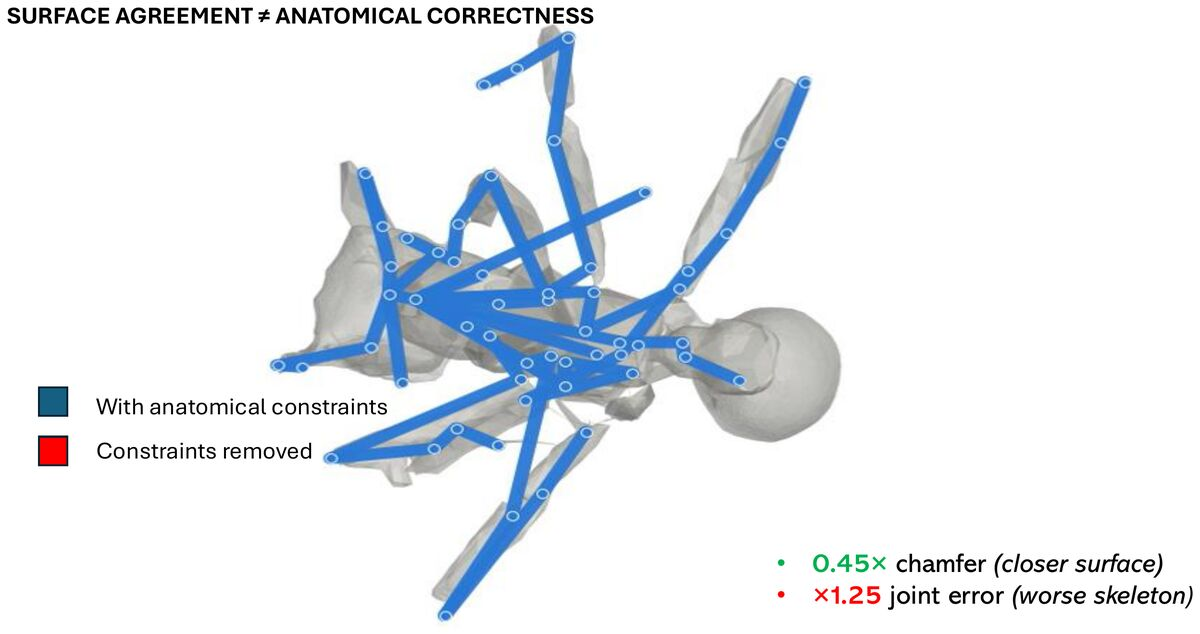
\includegraphics[width=\linewidth]{figures/fig_geometric_agreement.jpg}
\end{minipage}\hfill
\begin{minipage}[b]{0.46\linewidth}
\centering
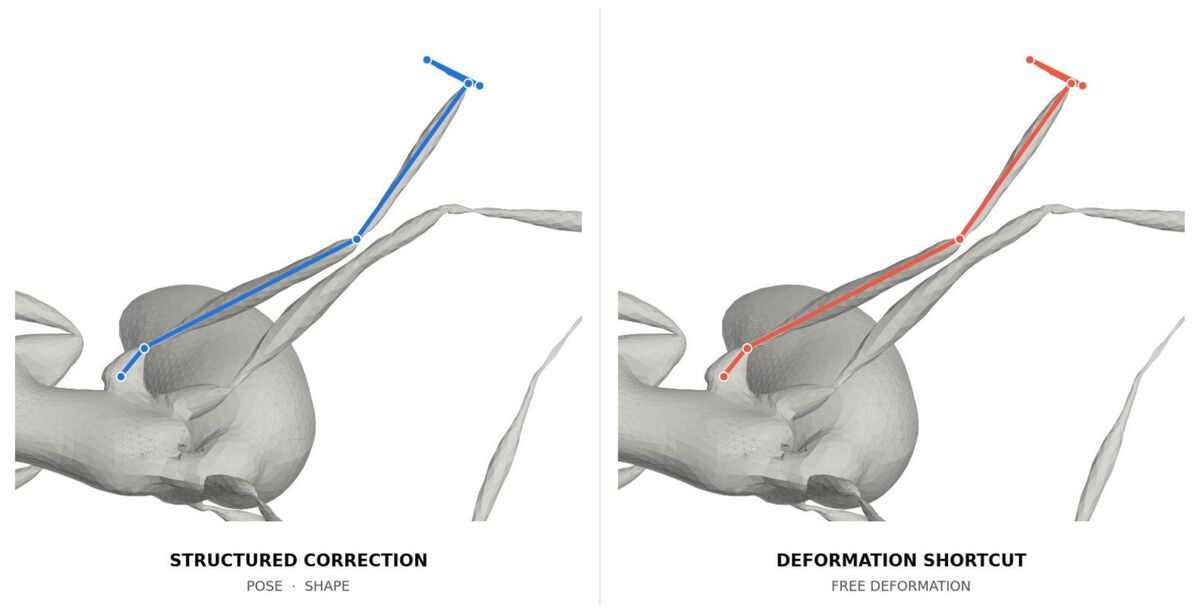
\includegraphics[width=\linewidth]{figures/fig_deformation_shortcut.jpg}
\end{minipage}
\caption[Surface agreement and the deformation shortcut]{Left: removing the
offset and normal penalties yields a closer surface and a worse skeleton
(skeleton overlay in blue shown with the penalties active). Right: a constructed
illustration of the mechanism, not a fit comparison, in which the same visual improvement is reached
by free per-vertex deformation that bends the leg, instead of re-posing the
joint.}
\label{fig:geometric-agreement}
\end{figure}

\subsection{What information is missing? Interrogating the explanation (RQ3)}
\label{sec:diagnosis}

If the objective cannot tell a correct explanation from a plausible one, the
natural question is which additional information would, and where it must be
supplied. Each experiment below supplies one kind of information, or one
counterfactual, and asks how much of the failure remains.

\subsubsection{Counterfactuals: how much is solved if one piece is given?}
\label{sec:oracle}

An \emph{oracle intervention} supplies the fitter with the correct answer to
exactly one sub-question, and the residual error then localises the bottleneck
without proposing a deployable fix (Table~\ref{tab:oracles}). Each oracle is a
minimal change to Equation~\eqref{eq:objective}: the \emph{regional} oracle
replaces the global Chamfer term by one computed within ground-truth region
labels; the \emph{dense} oracle adds
$w_{\mathrm{d}}\sum_{y\in Y}\|y-v_{\pi^\ast(y)}\|^2$, which matches each target
point to the fitted mesh's own vertex at its true index $\pi^\ast(y)$; and the
\emph{joint} oracle adds $\lambda\sum_j\|J_j(\bm\beta,\bm\theta,s)-J^\ast_j\|$
with $\lambda=0.03$. Because each oracle supplies strictly more of the
information that Equation~\eqref{eq:objective} lacks, the three form a ladder
from identity of a region, to identity of a vertex, to position of a joint. Supplying the
true region of every target point raises accuracy only partially, and most of
the gain comes from a minority of specimens; supplying exact per-vertex
correspondence improves within-part (segment-level) accuracy on every specimen
but remains clearly below the metric's own ceiling. Regional identity and
within-region localisation are therefore distinct problems (\F{F3}), and
correspondence is not the only missing ingredient: the objective, the
optimisation trajectory and the deformation freedom keep limiting the fit even
when correspondence is solved. The third oracle, expert joint positions, is the
only one on real data (Section~\ref{sec:skeleton}).

\begin{table}[!htb]
\centering
\caption{Oracle interventions, ordered by the amount of information supplied.}
\label{tab:oracles}
\begin{tabular}{@{}L{0.18\linewidth}L{0.18\linewidth}L{0.30\linewidth}L{0.26\linewidth}@{}}
\toprule
\textbf{Oracle} & \textbf{Supplied} & \textbf{What remains} & \textbf{Data}\\
\midrule
Regional identity & Which structure & Error \emph{inside} the correct
 structure & Synthetic, $n=12$\\
Dense correspondence & Where, per vertex & Objective, deformation and
 trajectory effects & Synthetic, $n=12$\\
Expert joints & True skeleton & No propagation to unsupervised regions &
 Real, $n=11$\\
\bottomrule
\end{tabular}
\end{table}

\subsubsection{Initialisation and articulation}
\label{sec:articulation}

\textbf{Question.} Is failure a matter of starting in the wrong basin?
Starting from the ground-truth pose instead of the default recovers most of
the lost accuracy along the \emph{distal} chain (pretarsus error falls about
twelvefold) but leaves the coxa unchanged. A matched sweep that fixes the total
pose error and varies only \emph{where along the chain} it sits shows why
(Figure~\ref{fig:articulation-bars}): the same error is recoverable at the tip
and damaging at the base, because a proximal mistake propagates through every
joint downstream. Initialisation sensitivity is thus anatomically
heterogeneous (\F{F4}).

The coxa result should be read for its mechanism rather than for the body part.
The fitter seeds, but does not freeze, the pose, and it drifts away from the
ground-truth pose it is given in \emph{every} segment; the coxal error
correlates with the error in the per-joint scale parameters, not with pose
drift. Where an attachment point is determined jointly by pose, per-joint scale
and body shape, correct pose alone cannot fix it, because the parameters
trade against one another. This is a statement about under-determination, and
the coxa is its clearest instance. (On exact synthetic meshes the coxa also
carries a measurable floor from neighbouring-coxa ambiguity, so its apparent
error must be read above that floor.) The correlation does not establish
direction of causation.

\begin{figure}[!htb]
\centering
\begin{minipage}[b]{0.46\linewidth}
\centering
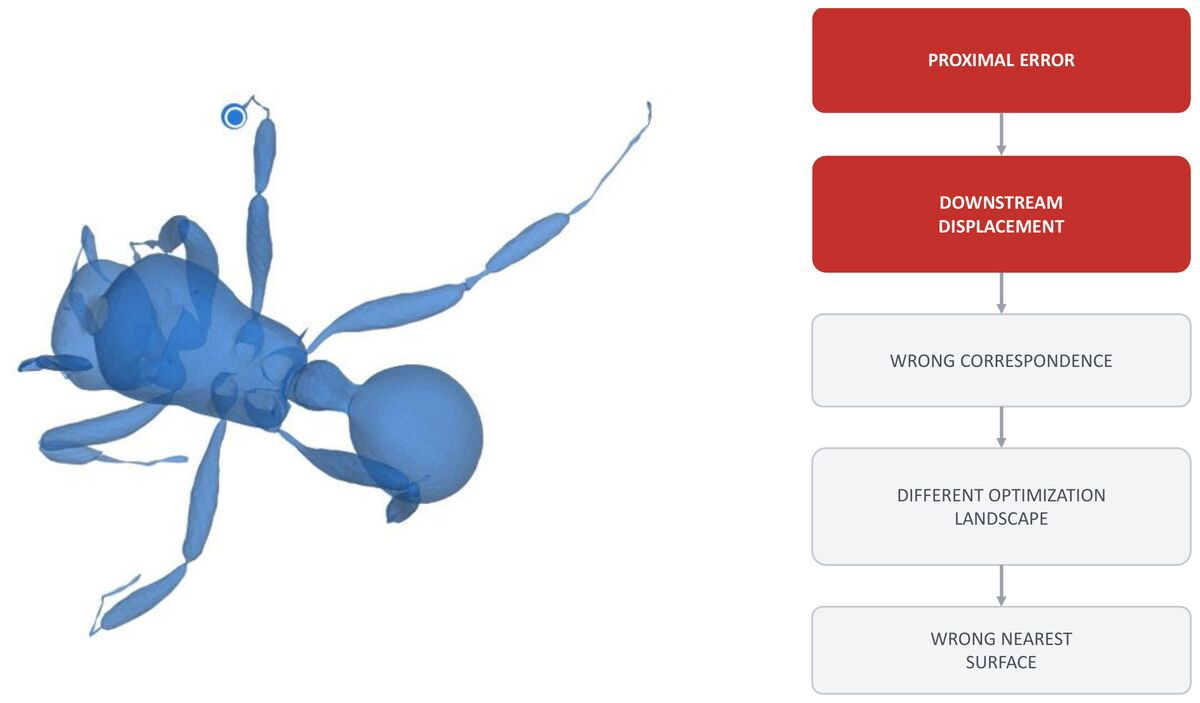
\includegraphics[width=\linewidth]{figures/fig_articulation_flow.jpg}
\end{minipage}\hfill
\begin{minipage}[b]{0.50\linewidth}
\centering
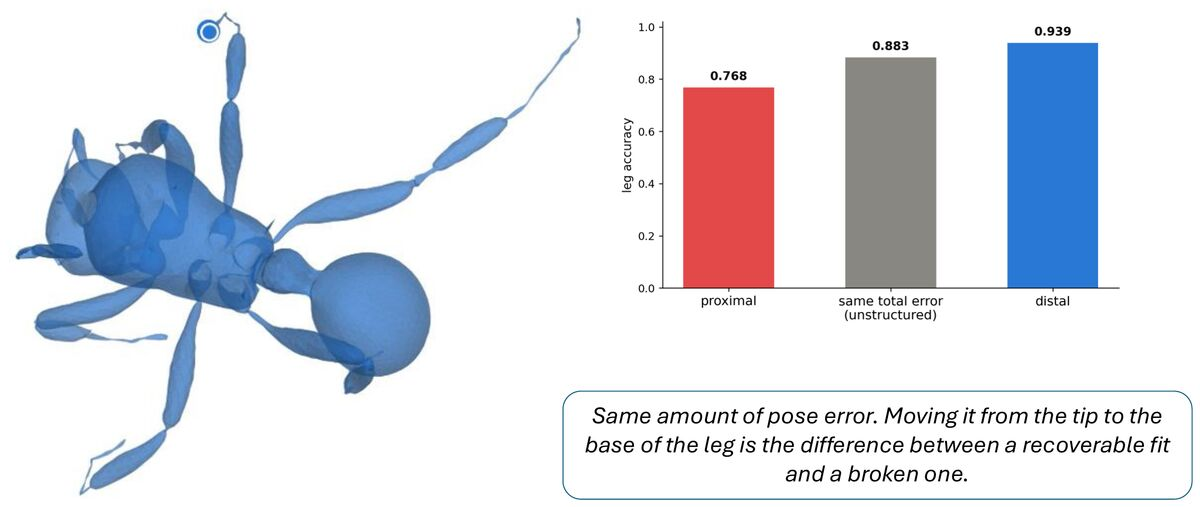
\includegraphics[width=\linewidth]{figures/fig_articulation_bars.jpg}
\end{minipage}
\caption[Pose error along the kinematic chain]{Left: a pose error near the
body propagates to everything distal to it. Right: leg accuracy for the same
total pose error placed at different points of the chain (synthetic, one seed
per condition): distal $0.94$, proximal $0.77$.}
\label{fig:articulation-bars}
\end{figure}

\textbf{A learned initialiser.} A PointNet-style encoder~\cite{pointnet} that
predicts pose, shape and global transform directly from the target was the
natural remedy. It wins clearly on synthetic data. On 50 real specimens, trained at the
synthetic perturbation magnitude, it is significantly \emph{worse} than the
default, and a controlled sweep of that magnitude moves it monotonically to
parity, which identifies a synthetic-to-real distribution mismatch as the
operative factor and locates the remedy in a more representative training
distribution, not in the architecture. The general rule is that a synthetic
evaluation cannot certify real-world transfer by itself. The pattern recurs in
the JAB: learned initialisation is neutral on most specimens and decisive, in
the wrong direction, on a few.

\subsubsection{Anatomical structure, sampling and robust optimisation}
\label{sec:sampling}

\textbf{Anatomical structure.} The Shape Diameter Function~\cite{sdf} assigns
each surface point a pose-independent thickness value and separates body from
appendage reliably (AUC $\approx0.97$). Separating \emph{instances} requires laterality, which local thickness does
not encode: on real scans the two mandibles fell into one connected component in
$9$ of $12$ specimens, because connected components cannot split structures
that are fused in the scan. This
matches a known limitation: intrinsic descriptors cannot distinguish a shape
from its mirror image, which is why orientation-aware formulations were
developed~\cite{donati}. Joint limits and bilateral symmetry improve
plausibility but not correspondence, and a Gaussian shape prior added as a
stabiliser was removed after it suppressed genuine variation. In each case the
information supplied constrained plausibility, not identity.

\textbf{Sampling.} The surface term is a Monte Carlo estimate over sampled
points, so the sampling distribution is an implicit weighting over anatomy.
The template supports a coxa or trochanter with $200$--$275$ vertices but a
tarsus with $38$ and a pretarsus with only $8$ (counted by dominant skinning
weight for one leg), so a thin distal structure is almost invisible to the
optimiser (\F{F5}). Reserving a sampling quota for distal points helped the legs
but starved the antennae and head. Starvation is a real confound, but
controlling it did not create anatomical correspondence.

\textbf{Robust optimisation.} Graduated non-convexity (GNC)~\cite{gnc} treats
every match as suspect at first and hardens its confidence as optimisation
proceeds. Applied to the whole body it distorted the antennae; restricted to the leg
points it improved synthetic-corruption scores. The metric behind that early
gain was a mismatch fraction whose definition has since been corrected, and the
clean-data version did not reproduce under a paired bootstrap. GNC is therefore
carried as a candidate with a defined verification protocol (leg and segment
accuracy under the damage corpora), not as a shipped component.

\subsubsection{Correspondence learned from data}
\label{sec:learned-correspondence}

\textbf{Question.} Can a descriptor trained for the task do what geometry
cannot? Normalising points within their anatomical part performed \emph{worse}
than raw coordinates, since normalising away a part's geometry removes signal.
A first learned descriptor was undone at deployment by a mismatch between the
point density it was trained and evaluated on. A within-part,
context-trained descriptor then beat part-local rigid proximity at the coxa, the
one place where rigid proximity is least informative, and nowhere else, and the gain grew with
training: a learned local descriptor does carry information that raw geometry
does not.

Two tasks must nevertheless be kept apart. \emph{Pairwise retrieval} matches
each query point to its nearest neighbour in descriptor space; \emph{dense
correspondence} needs a whole assignment that is globally consistent and covers
the surface. Deployed in the form the fitter consumes, the same descriptor
lost on every one of 48 specimens against the existing key-table method, and
its votes collapsed onto a few template vertices (coverage of coxal vertices
$1.8\%$ against $28.1\%$; Figure~\ref{fig:local-vs-global}). Restricting the
baseline to the descriptor's own candidate set changed the result by only a few
per cent, so the gap is not an artefact of the comparison. Local accuracy does
not imply global consistency. This is the benchmark-versus-system gap that
machine-learning evaluation work calls a gap in external
validity~\cite{liao}, and it points to what is missing: a mechanism that
couples the votes into one consistent assignment (Section~\ref{sec:conclusion}).
The same bimodality appears in the JAB, where a learned dense correspondence
head produced large wins on some specimens and large losses on others, and a
prediction made in advance by the correspondence-distribution literature, that
ambiguity on symmetric surfaces should show up as multi-modality~\cite{haugaard}.

\begin{figure}[!htb]
\centering
\begin{tikzpicture}[every node/.style={font=\small},
 n/.style={draw,rounded corners=2pt,minimum height=6.5mm,align=center,fill=white,inner sep=3pt,text width=5.6cm}]
\node[n,fill=green!12] (a) {\textbf{Local test}};
\node[n,below=2mm of a] (a2) {within-part descriptor, better pairwise retrieval};
\node[n,below=2mm of a2,fill=green!12] (a4) {gain over rigid proximity at the coxa};
\node[n,right=10mm of a,fill=red!10] (b) {\textbf{Deployment}};
\node[n,below=2mm of b] (b2) {dense correspondence field, votes collapse};
\node[n,below=2mm of b2,fill=red!10] (b4) {coverage $28.1\%\to1.8\%$};
\end{tikzpicture}
\caption[Local success versus global consistency]{The same descriptor at two
levels: strong local retrieval does not imply a usable dense correspondence
field.}
\label{fig:local-vs-global}
\end{figure}

\subsubsection{The objective does not constrain skeleton position}
\label{sec:skeleton}

\textbf{Question.} Is there a better skeleton within the model's reach, and if
so why does the optimiser not find it? Production joint error is about a
quarter of Weber's length (median $25.1\%$, 95\% CI $17.5$--$44.8$). Supplying
expert joint targets during fitting lowers it to $17.4\%$ against the same
specimens' own baseline ($10$ of $11$ improve), so a better skeleton exists
within the model's own shape budget. Yet no single-factor change to the shipped
recipe improves joint alignment reliably, and the shipped recipe ranks best of
the twelve (Table~\ref{tab:jab}). Supervision supplied everywhere \emph{except}
one region leaves that region essentially unchanged, with every held-out
interval including zero. The production objective therefore contains no
explicit observation of joint location and constrains the skeleton only
indirectly; supervision acts locally and does not propagate (\F{F6}). Within
the pipeline, alignment is largely won in one place, the hierarchical leg
stage, which improved all eleven specimens, while later steps add little.
Reweighting terms that do not measure the missing quantity cannot recover it.
The scale cap and allometric prior shipped to curb scale outliers are
joint-neutral; they fixed a statistic rather than the anatomy.

The error is structured, not uniform (Figure~\ref{fig:structured-error}):
proximal leg joints are placed at about $12$--$13\%$ of WL, the body axis at
$24\%$, and mandibles, antennae and distal leg segments at $43$--$56\%$. A
variance decomposition attributes far more of the spread to \emph{which joint}
and \emph{which specimen} than to the optimiser seed (\F{F8}), so failure is
anatomically structured and not a matter of luck. The hierarchy is the expected
one: hand-pose benchmarks have long reported error growing along a kinematic
chain, so the ordering is not claimed as a finding; what is new is the usable
per-region number.

\begin{table}[!htb]
\centering
\caption{Joint Alignment Benchmark: selected strategies against the shipped
recipe (A). Joint-level ratio $>1$ means a worse skeleton; $\Delta$ is the
paired median shift in \% of WL ($n=11$).}
\label{tab:jab}
\begin{tabular}{@{}L{0.33\linewidth}cccc@{}}
\toprule
\textbf{Strategy} & \textbf{Median} & $\Delta$ \textbf{vs A} & \textbf{Joint-level} & \textbf{Chamfer}\\
 & (\% WL) & (worse/better) & \textbf{ratio} & \textbf{vs A}\\
\midrule
A\; shipped recipe & 25.1 & --- & --- & $1.00\times$\\
B\; no hierarchical placement & 37.9 & $+8.2$ (10/1) & 1.23 & $1.19\times$\\
D\; no joint limits & 29.9 & $+4.0$ (9/2) & 1.05 & $0.96\times$\\
F\; no scale cap & 26.0 & $+0.5$ & 1.01 & $1.00\times$\\
G\; allometric prior & 25.8 & $0.0$ & 0.99 & $1.00\times$\\
I\; learned correspondence & 25.3 & $+2.3$ (bimodal) & 1.08 & $2.97\times$\\
J\; no offset/normal penalty & 32.7 & $+5.0$ (8/3) & 1.25 & $0.45\times$\\
K\; pose frozen & 29.3 & $+3.8$ (9/2) & 1.18 & $2.18\times$\\
\bottomrule
\end{tabular}
\end{table}

\begin{figure}[!htb]
\centering
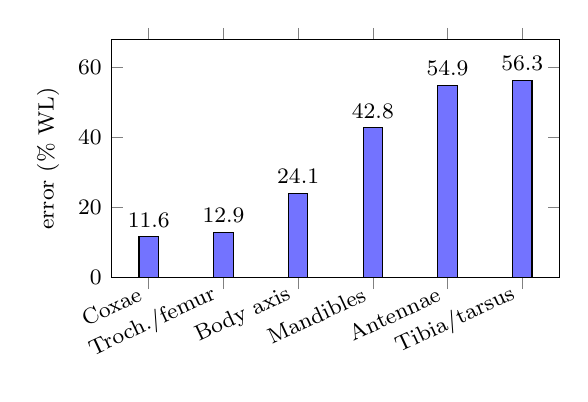
\begin{tikzpicture}
\begin{axis}[ybar,width=0.60\linewidth,height=4.6cm,bar width=7pt,ymin=0,ymax=68,
 symbolic x coords={Coxae,Troch./femur,Body axis,Mandibles,Antennae,Tibia/tarsus},
 xtick=data,x tick label style={rotate=25,anchor=east,font=\footnotesize},
 ylabel={error (\% WL)},ylabel style={font=\footnotesize},tick label style={font=\footnotesize},
 nodes near coords,every node near coord/.append style={font=\footnotesize}]
\addplot[fill=blue!55] coordinates {(Coxae,11.6)(Troch./femur,12.9)(Body axis,24.1)(Mandibles,42.8)(Antennae,54.9)(Tibia/tarsus,56.3)};
\end{axis}
\end{tikzpicture}
\hfill
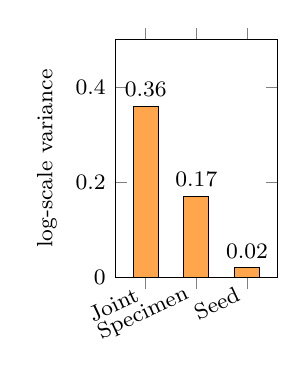
\begin{tikzpicture}
\begin{axis}[ybar,width=0.30\linewidth,height=4.6cm,bar width=9pt,ymin=0,ymax=0.5,
 enlarge x limits=0.3,
 symbolic x coords={Joint,Specimen,Seed},xtick=data,tick label style={font=\footnotesize},
 x tick label style={rotate=25,anchor=east},
 ylabel={log-scale variance},ylabel style={font=\footnotesize},nodes near coords,
 every node near coord/.append style={font=\footnotesize,/pgf/number format/fixed,/pgf/number format/precision=2}]
\addplot[fill=orange!70] coordinates {(Joint,0.36)(Specimen,0.17)(Seed,0.02)};
\end{axis}
\end{tikzpicture}
\caption[Structure of the skeleton error]{Left: median skeleton error by region
for the shipped recipe. Right: variance decomposition across the same fits; the
optimiser seed contributes almost nothing.}
\label{fig:structured-error}
\end{figure}

\subsection{From registration to measurement validity (RQ4)}
\label{sec:measurement}

\textbf{Question.} When a parameter is recovered, when is it a valid biological
measurement? A fitted model is an instrument, and an instrument is judged
against an independent reference. Manual joint annotation by an expert provides
one for the skeleton (Figure~\ref{fig:ground-truth}, left), and a physical
head-width reference provides one for a trait.

\begin{figure}[!htb]
\centering
\begin{minipage}[b]{0.50\linewidth}
\centering
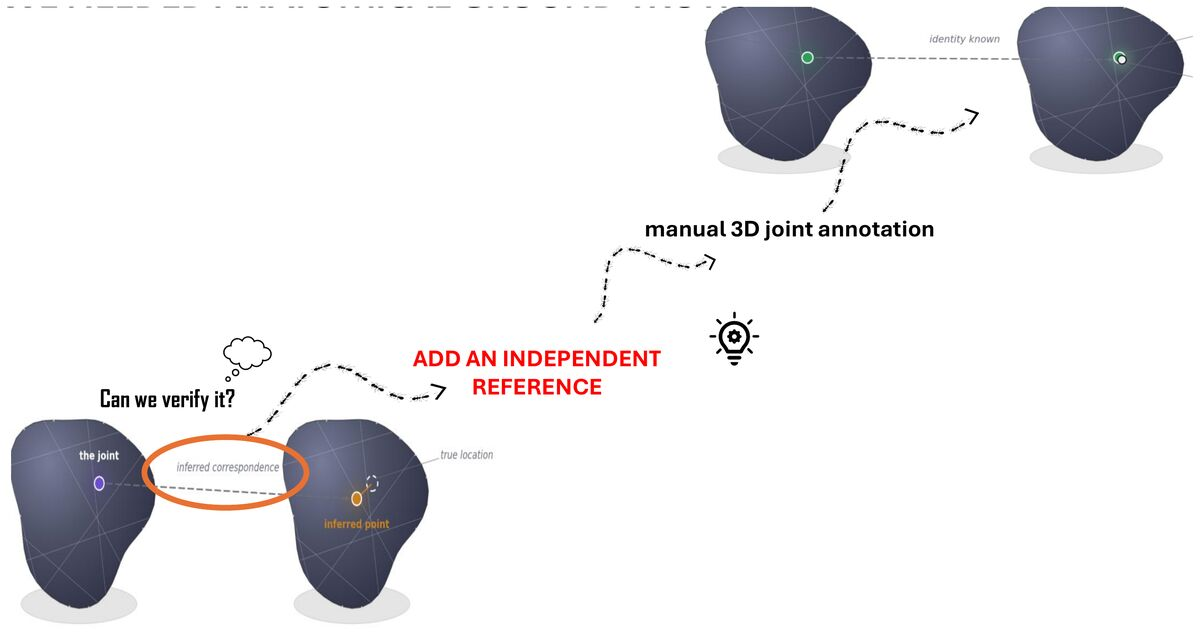
\includegraphics[width=\linewidth]{figures/fig_ground_truth_annotation.jpg}
\end{minipage}\hfill
\begin{minipage}[b]{0.38\linewidth}
\centering
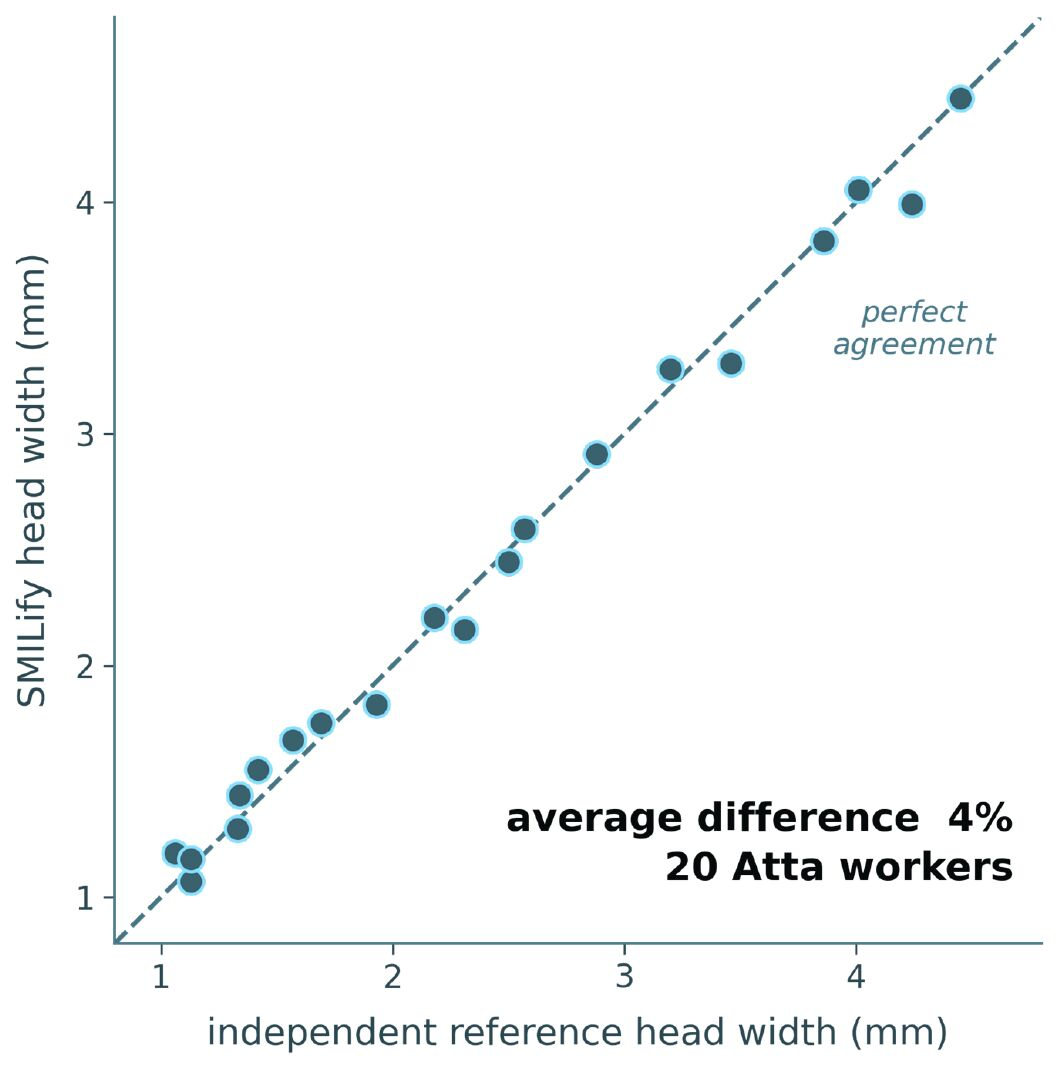
\includegraphics[width=\linewidth]{figures/fig_parameter_measurement.jpg}
\end{minipage}
\caption[Independent references]{Left: manual 3D joint annotation as an
independent reference, with identity known by construction. Right: head width
read from 20 fitted \emph{Atta} workers against a reference measurement.}
\label{fig:ground-truth}
\end{figure}

\textbf{A trait that survives.} Head width, read from two reporter bones placed
on the head, agrees with the reference on 20 \emph{Atta} workers with a mean
absolute difference of about $4\%$ and reproduces the allometric slope against
mass closely. Agreement in millimetres is partly built in, because scale is
restored from body length; the dimensionless ratio of head width to body length
is the more informative test, and it also agrees. The result is deliberately
narrow: one trait, one species, $n=20$, and whether the reference widths were
measured or estimated is still to be confirmed. An earlier, tighter figure
could not be reproduced and is not used.

\textbf{What does not.} Registration of an independent ethanol-preserved worker
corpus sits at a measurable noise floor, at which two conspecific workers are
only about $7\%$ closer than unrelated ants, and distal leg and antenna
segment lengths, the structures the expert benchmark and the sampling audit
already identify as least reliable, disagree between nest-mates more than
random ants do. A synthetic reliability table, the earlier basis for choosing trustworthy
measurements, was compared with real annotations for the first time on the
earlier annotation set; that comparison is to be repeated on the corrected
benchmark, and until then region-level reliability is taken from the benchmark
itself. Genus-level structure in shape-ratio traits is reported as an
exploratory population-level result.

Taken together, ``the registration is valid'' is not one claim but four, holding
at different scales and supported by different evidence (Table~\ref{tab:validity}).
A model can give an accurate population-level or single-trait measurement while
failing to preserve the individual-level correspondence needed for
specimen-by-specimen comparison, and each statement is supported only at its own
level. The expert-supervised fit quantifies the headroom available; since expert
joints are unavailable at inference time, supplying an equivalent signal
automatically is the objective it motivates.

\begin{table}[!htb]
\centering
\caption{Four levels of registration validity and the evidence for each.}
\label{tab:validity}
\begin{tabular}{@{}L{0.20\linewidth}L{0.34\linewidth}L{0.34\linewidth}@{}}
\toprule
\textbf{Level} & \textbf{Question} & \textbf{Evidence}\\
\midrule
Surface correspondence & Are the surfaces close? & Chamfer, F-score
 (misleading alone, \F{F1})\\
Anatomical correspondence & Does vertex $i$ mark the same structure across
 specimens? & Synthetic oracles, expert benchmark (\F{F3}, \F{F6})\\
Parametric correspondence & Do $\bm\beta,\bm\theta$ mean the same thing across
 specimens? & Only partially established; nest-mate agreement low\\
Measurement validity & Does a derived measurement match an independent one? &
 \emph{Atta} head width\\
\bottomrule
\end{tabular}
\end{table}

\subsection{Summary of findings and evidence status}
\label{sec:ledger}

The results that recur are registered once and cited by identifier
(Table~\ref{tab:findings}). Beyond them, the evidence status is: the scale cap is a validated
proxy fix whose anatomical mechanism was tested and found null; robust
optimisation is a candidate with a defined verification protocol; trait
reliability and genus-level structure await re-evaluation on the corrected
benchmark; and functional maps, optimal transport and canonical anatomical
fields are the directions the findings point to.

\begin{table}[!htb]
\centering
\caption{Findings ledger: the load-bearing results and their evidence status.}
\label{tab:findings}
\printfindingledger
\end{table}
